\documentclass{article}

% if you need to pass options to natbib, use, e.g.:
% \PassOptionsToPackage{numbers, compress}{natbib}
% before loading nips_2017
%
% to avoid loading the natbib package, add option nonatbib:
% \usepackage[nonatbib]{nips_2017}

\usepackage[final]{nips_2017}


\usepackage[utf8]{inputenc} % allow utf-8 input
\usepackage[T1]{fontenc}    % use 8-bit T1 fonts
\usepackage{hyperref}       % hyperlinks
\usepackage{url}            % simple URL typesetting
\usepackage{booktabs}       % professional-quality tables
\usepackage{amsfonts}       % blackboard math symbols
\usepackage{nicefrac}       % compact symbols for 1/2, etc.
\usepackage{microtype}      % microtypography
\usepackage{graphicx}
% Choose a title for your submission
\title{Your title here}


\author{Student 1 \qquad Student 2 \qquad Sandar Felicity Lim}
\graphicspath{ {fig/} }
\begin{document}
% \nipsfinalcopy is no longer used

\maketitle

% We do not requrire you to write an abstract. Still, if you feel like it, please do so.
%\begin{abstract}
%\end{abstract}

Feel free to add more sections but those listed here are strongly recommended.
\section{Introduction}
You can keep this short. Ideally you introduce the task already in a way that highlights the difficulties  your method will tackle.

\section{Methodology}
\subsection{Generating wrong endings}
Wrong endings were generated for each story to better train our classifier. Naive way would be to randomize the correct endings of each story. However, doing so would obviously change the main charecter or main point of the story. Therefore, we needed to generate endings that are wrong but still preserves narrative structure. Negation of the fifth sentence was a promising way to achieve that end. i.e. The resulting sentence would be contain at least one of the charecters of the story. The resulting sentence would still be generally realisitic, except that it would not create a meaningful story as an addition to the previous four sentences.

Negation can be challenging for complex sentence structures because we would have to decide which part of the sentence to negate. For example, the sentence: "
Kelly quickly went home." There are two possibilities of negation: "Kelly slowly went home", "Kelly did not quickly go home". If we do not keep track the number of negations in the sentence, the result would be "Kelly did not slowly go home". Hence, our approach was to first negate the adjectives and adverbs, and in their absence, negate the verbs, all the while keeping count of number of negations in the generated sentence.

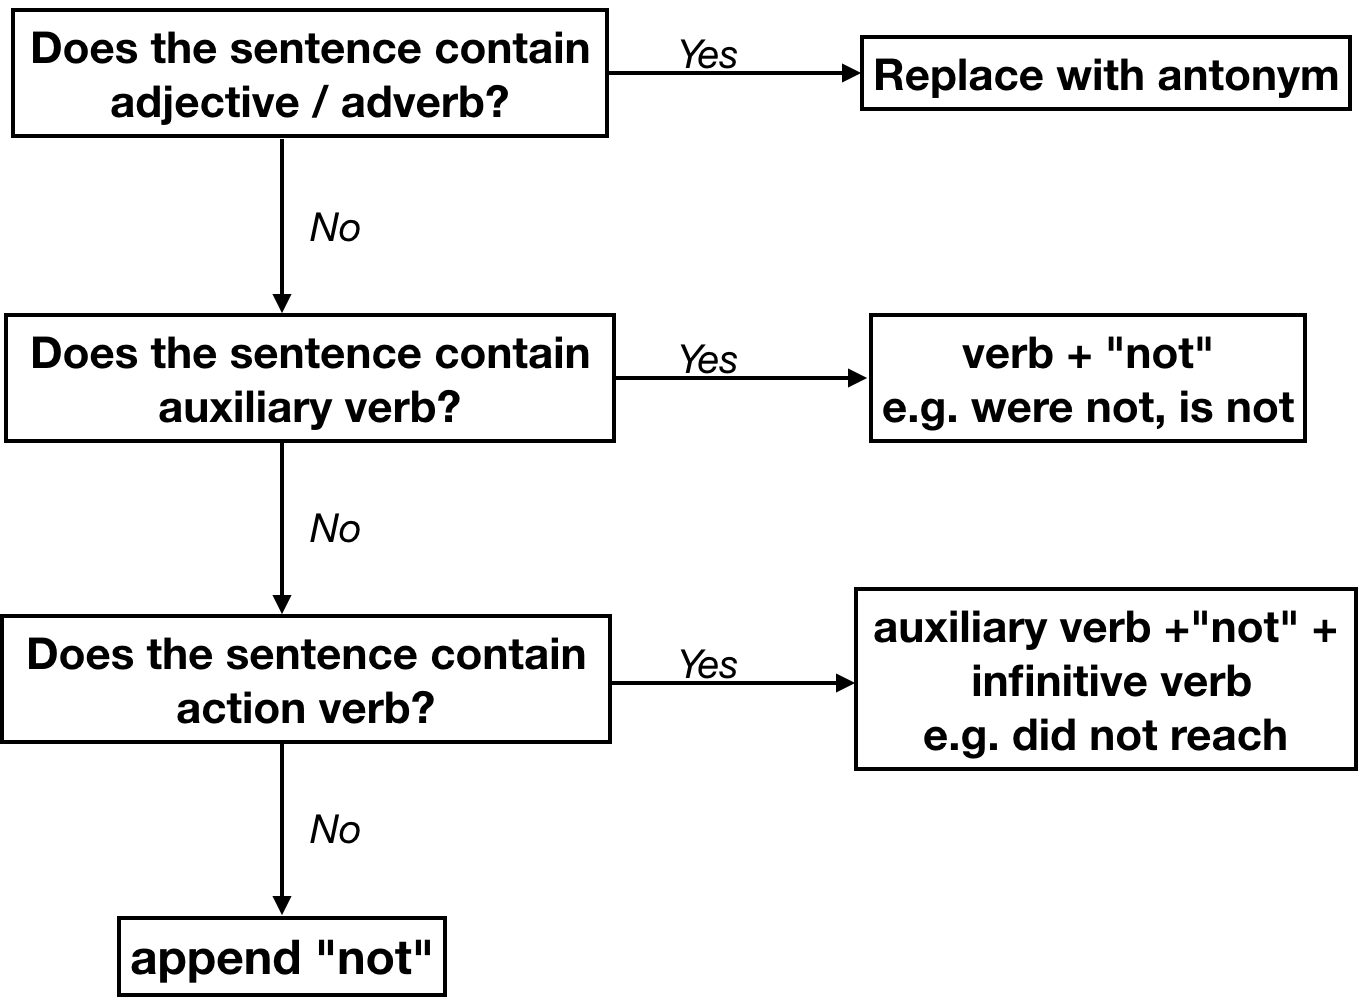
\includegraphics[width=0.9 \linewidth]{wrong.PNG}


A few examples of our successful sentence generations are



Kelly found her grandmother's pizza recipe in a shoebox of memories.,Kelly reminisced about how much she loved her grandmother's pizza.,Kelly decided that she was going to try to make pizza.,Kelly studied the recipe and gathered everything she needed.,Kelly successfully made a pizza from her grandmother's recipe., Kelly unsuccessfully made a pizza from her grandmother 's recipe .,Kelly unsuccessfully made a pizza from her grandmother 's recipe .




strange: ,Tom hit a watery oily patch.,He spun out of control and hit a tree.,Tom was paralyzed from the neck down., Tom was not paralyzed from the neck down .,Tom was not paralyzed from the neck down .,Tom was paralyzed from the neck down.,Tom was not paralyzed from the neck down .,1

Too Much Candy,Laura found a jar of candy in her mom's kitchen.,Laura ate all of the candy.,She got really sick.,Laura's mom discovered why Laura was sick.,Her mom felt bad for her so she didn't punish her for eating it all., Her mom felt good for her so she did n't punish her for eating it all .,Her mom felt good for her so she did n't punish her for eating it all .,Her mom felt bad for her so she didn't punish her for eating it all.,Her mom felt good for her so she did n't punish her for eating it all .,1

3add804c-4935-41fd-baf7-21b86f08151d,My girlfriend works too much,I made plans for dinner with my girlfriend.,She agreed to go to dinner with me.,We were on our way to a nice restaurant.,She got a phone call from work.,"We had to cancel dinner so she could go into work,"," We did not have to cancel dinner so she could go into work ,","We did not have to cancel dinner so she could go into work ,","We did not have to cancel dinner so she could go into work ,","We had to cancel dinner so she could go into work,",2


3039b5e6-7aae-4e52-b6e1-2182de70a65e,Planting a Garden,Every spring I make a garden.,I go to the store and buy seeds.,At home I get out my garden tools.,I dig up the dirt and pull weeds.,I plant the seeds and water them., I plant the seeds and water them .,I plant the seeds and water them not.,I plant the seeds and water them not.,I plant the seeds and water them.,2


did not work:
Once he grew up he realized he wanted to do other things.,His dad was very angry.,Their relationship got bad and they no longer talked., Their relationship got good and they no longer talked .,Their relationship got good and they no longer talked .,Their relationship got good and they no longer talked .,Their relationship got bad and they no longer talked.,2


f10eba84-f7b4-44df-897e-6927538e0050,Dog fight.,When walking home from a convenient store I noticed two dogs.,At first they didn't do much.,"Then, out of nowhere they started attacking each other.","I tried breaking the fight at first, but I couldn't by myself.",Me and the neighbors eventually pulled the dogs away from each other., Me and the neighbors eventually pulled the dogs home from each other .,Me and the neighbors eventually pulled the dogs home from each other .,Me and the neighbors eventually pulled the dogs home from each other .,Me and the neighbors eventually pulled the dogs away from each other.,2
cbf6d8ff-b21f-483c-9883-cd2f99c3ccfa,The Date Nerves,Emily was going on a first date


25438bdc-2b79-4f57-ab33-8406018619e9,Dress,I was shopping for a dress for my daughter.,I wanted to find something that fit her personality.,"She is very creative, so I looked for something unusual.",I found a dress that was red and had pretend paint splatters.,"I went home happy, having found the perfect dress."," I went home happy , having found the imperfect dress .","I went home happy , having found the imperfect dress .","I went home happy, having found the perfect dress.","I went home happy , having found the imperfect dress .",1

15e11d39-53b0-4242-a345-6f8c709917bb,Parties,Anna was invited to two parties on weekend.,One was being thrown by the popular crowd she adored.,The other was being thrown by her long-time friends.,Anna wished she could attend the popular party.,But she knew the right thing to do was attend her friends' party., But she knew the left thing to do was attend her friends ' party .,But she knew the left thing to do was attend her friends ' party .,But she knew the left thing to do was attend her friends ' party .,But she knew the right thing to do was attend her friends' party.,2

works:
0440d713-98c7-494a-9021-98750467a5f9,Tumbling Down,Tim was hiking up a mountain with friends.,He wasn't paying attention and lost his footing.,Tim tumbled down down for a few yards.,He was severely hurt.,Tim's friends had to call for help and carry him., Tim 's friends did not have to call for help and carry him .,Tim 's friends did not have to call for help and carry him .,Tim 's friends did not have to call for help and carry him .,Tim's friends had to call for help and carry him.

01cd5b80-7da8-481b-a9ec-c3964c08af14,The Doorbell,The family was tired of not hearing when someone knocked on their door.,They installed a doorbell on their front door.,It would ring a pleasant tune when someone came to see them.,They never missed houseguests anymore.,The family wished they'd gotten the doorbell earlier!, The family wished they 'd gotten the doorbell late !,The family wished they 'd gotten the doorbell late !,The family wished they 'd gotten the doorbell late !,The family wished they'd gotten the doorbell earlier!,2


b425930e-fcee-474c-98f2-522b2608d48a,Bea in the Lobby,My sister-in-law Bea rarely goes out into the lobby.,She drives her car into the garage and goes home.,Today we were shocked.,Bea was in the lobby.,She was waiting for a friend., She was not waiting for a friend .,She was not waiting for a friend .,She was waiting for a friend.,She was not waiting for a friend .,1

63a1ed11-4eb9-4ae8-ad7b-8928f30a36c9,Mango,She had a sudden craving for mangoes.,She went to the store looking for some.,She found some that were very ripe.,The sweet flavor was pungent and satisfying.,She ate them for every meal that day., She did not eat them for every meal that day .,She did not eat them for every meal that day .,She ate them for every meal that day.,She did not eat them for every meal that day .,1
\section{Model}
The math/architecture of your model. This should formally describe your idea from above. If you really want to, you can merge the two sections.
\section{Training}
What is your objective? How do you optimize it?

\section{Experiments}
This {\bf must} at least include the accuracy of your method on the validation set.
\section{Conclusion}
You can keep this short, too.
\end{document}
